\chapter{Requirements, Use Cases and Testing}\label{ch:style}

This chapter aims to outline the project's requirements, use cases, and testing methodology. Further changes will be made in thesis part B \& C upon discovering new requirements or evaluating feedback from testing. 

\section{Requirements}
The following requirements are done in correspondence to MoSCoW requirement structure:
\begin{itemize}
    \item P1 (Priority 1, must have)
    \begin{itemize}
        \item All these requirements form the MVP and are crucial for launch
    \end{itemize}
    \item P2 (Priority 2, should have)
    \begin{itemize}
        \item All these requirements should be done within the time frame but are not crucial to launch and can be delayed to further releases
    \end{itemize}    
    \item P3 (Priority 3, could have)
    \begin{itemize}
        \item All these requirements are featured we would like but in the time frame we would delay these to focus on priorities 1 and 2
    \end{itemize}
    \item P4 (Priority 4, would have)
    \begin{itemize}
        \item Features we do not expect to have but show potential extensions of our product.
    \end{itemize}     
\end{itemize}

\begin{enumerate}


    \item[1.] \textbf{I will create an algorithm that is able to detects falls. [P1]}
    \begin{enumerate}[label*=\arabic*.]
        \item[1.1.] I will create a deep learning model that is able to detect falls. \textbf{[P1]}
        \begin{enumerate}[label*=\arabic*.]
            \item[1.1.1.] I will create a deep learning model that is able to detect ADL \textbf{[P1]}
            \begin{enumerate}[label*=\arabic*.]
                \item[1.1.1.1.] I will define ADL as a single output class and abnormalities as the other output class. \textbf{[P1]}
            \end{enumerate}
        \end{enumerate}

    \end{enumerate}
   \begin{enumerate}[label*=\arabic*.]
        \item[1.2.] I will create a generative model that can compute the probability of an event being generated with the input given. \textbf{[P1]}
        \begin{enumerate}[label*=\arabic*.]
            \item[1.2.1.] I will create a function that is able to under sample abundant ADL data and oversample lacking fall data. \textbf{[P1]}
            \item[1.2.2.] I will create a model that contains A Variational Autoencoder to encode inputs. \textbf{[P1]}
            \item[1.2.3.] I will create a model that connects the encoder from requirement 1.2.2 to a LSTM to process the encoded inputs. \textbf{[P1]}
            \item[1.2.4.] I will create a model that connects the outputs from requirement 1.2.3 to a decoder to determine likelihood of reconstruction. \textbf{[P1]}
            \item[1.2.5.] I will set a threshold to trigger for abnormality based on the output of requirement 1.2.4. \textbf{[P1]}
        \end{enumerate}
    \end{enumerate}  
    
       \begin{enumerate}[label*=\arabic*.]
        \item[1.3.] I will create a function that is triggered on requirement 1.2.5 that will check more detailed information on the abnormality. \textbf{[P1]}
        \begin{enumerate}[label*=\arabic*.]
            \item[1.3.1] I will create a function that determines the velocity and difference in centroid height and compares to a set threshold. \textbf{[P1]}
            \begin{enumerate}[label*=\arabic*.]
                \item[1.3.1.1.] I will create a function that triggers an alert from requirement 1.3.1. \textbf{[P1]}
            \end{enumerate}
        \end{enumerate}
    \end{enumerate}  
    
    
    \item[2.] \textbf{I will collect data from mmWave Radars. [P1]}
    \begin{enumerate}[label*=\arabic*.]
        \item[2.1.] Data will be processed locally. \textbf{[P1]}
        \begin{enumerate}[label*=\arabic*.]
            \item[2.1.1.] mmWave radar data will be cleaned to remove outliers, anomalies and incorrect camera values. \textbf{[P1]}
        \end{enumerate}
        \begin{enumerate}[label*=\arabic*.]
            \item[2.1.2.] mmWave radar data will be grouped to give XYZ coordinates, Doppler information. \textbf{[P1]}
        \end{enumerate}
        \begin{enumerate}[label*=\arabic*.]
            \item[2.1.3.] mmWave radar data will be processed to distinguish multiple people in a frame. \textbf{[P3]}
        \end{enumerate}
    \end{enumerate}
    \begin{enumerate}[label*=\arabic*.]
            \item[2.2.] Data will be collected locally on edge computers. \textbf{[P1]}
    \end{enumerate}
    \begin{enumerate}[label*=\arabic*.]
        \item[2.3.] Processed data will be sent to the model in real-time to detect falls. \textbf{[P1]}
        \begin{enumerate}[label*=\arabic*.]
            \item[2.3.1.] Processed data will be sent to the model through an edge computer, and the output of the model will be sent to an azure function. \textbf{[P1]}
        \end{enumerate}
    \end{enumerate}
    
    \item[3.] \textbf{I will create a backend system to detect falls as abnormalities in realtime. [P2]}
    \begin{enumerate}[label*=\arabic*.]
        \item[3.1.] I will create a backend system that works with requirement 2 in order to collect data. \textbf{[P2]}
    \end{enumerate}
    \begin{enumerate}[label*=\arabic*.]
        \item[3.2.] I will create a backend system to pass the collected data to the model in requirement 1. \textbf{[P2]}
    \end{enumerate}
    \begin{enumerate}[label*=\arabic*.]
        \item[3.3.] I will create a backend system that uses the alert from requirement 1.3.1.1 to alert a carer. \textbf{[P3]}
        \begin{enumerate}[label*=\arabic*.]
            \item[3.3.1.] I will create an azure function that is triggered upon requirement 1.3.1.1. \textbf{[P3]}
            \begin{enumerate}[label*=\arabic*.]
                \item[3.3.1.1.] I will create a function that sends an alert to a caretaker via SMS. \textbf{[P3]}
            \end{enumerate}
        \end{enumerate}
    \end{enumerate}
    
    \item[4.] \textbf{I will create a model that is able to detect other dangerous events such as seizures alongside requirement 1. [P4]}
    \begin{enumerate}[label*=\arabic*.]
        \item[4.1.] I will create further algorithms similar to requirement 1.3.1.1 that will be able to distinguish between different anomalies. \textbf{[P4]}
    \end{enumerate}
    \begin{enumerate}[label*=\arabic*.]
        \item[4.2.] Using the same system as Requirement 3, correct emergency contacts will be notified when specific abnormalities occur. \textbf{[P4]}
    \end{enumerate}
\end{enumerate}

\section{Use Cases}
The following use cases cover all priority 1 requirements as well as some priority 2 requirements
\begin{table}[H]
    \centering
    \begin{tabular}{ |p{2.8cm}|p{8cm}|}
     \hline
     \multicolumn{2}{|c|}{Use Case 1} \\
     \hline
      Requirements&1.3, 3.3\\
     \hline
     Outline &An alert is sent to an azure function that sends an SMS or phonecall to emergency contact upon fall detection.\\
     \hline
     Users&emergency contacts, falling individual, internal software.\\
     \hline
     Overview&Upon detecting a fall the system will send an alert to an azure function to signal that an individual has fallen over, the azure function will be designed to contact the emergency contact of choice for the individual.\\
     \hline
     Trigger&individual has fallen over.\\
     \hline
     Precondition&The model has returned that an individual has fallen.\\
     \hline
     Postcondition&The emergency contact has been notified and alerted.\\
     \hline
    \end{tabular}
\end{table}

\begin{table}[H]
    \centering
    \begin{tabular}{ |p{2.8cm}|p{8cm}|}
     \hline
     \multicolumn{2}{|c|}{Use Case 2} \\
     \hline
      Requirements&2\\
     \hline
     Outline &Data from mmWave radars are processed locally.\\
     \hline
     Users&internal software.\\
     \hline
     Overview&Upon installation of the system, mmWave radars begin automatically sensing objects nearby. The data collected is sent locally to an edge computer, where data processing occurs. Data is cleaned and to remove anomalies and outliers, and a python script begins processing the incoming data. information regarding the coordinates, doppler, and centroid are extracted and sent to the model in real-time.\\
     \hline
     Trigger&The system has been integrated.\\
     \hline
     Precondition&The equipment is satisfactory, and all hardware connections have been made.\\
     \hline
     Postcondition&Processed data is sent to the model in real time.\\
     \hline
    \end{tabular}
\end{table}

\begin{table}[H]
    \centering
    \begin{tabular}{ |p{2.8cm}|p{8cm}|}
     \hline
     \multicolumn{2}{|c|}{Use Case 3} \\
     \hline
      Requirements&1.2\\
     \hline
     Outline &Processed data is sent to the model in real time to classify each batch of frame inputs as a fall or not fall.\\
     \hline
     Users&Internal software.\\
     \hline
     Overview&The model has been trained and receives data in batches of frame using a sliding window approach. Upon detection of an abnormality from the batch, the model will perform further fall detection algorithms such as determining the motion of the subject in frame sequence.\\
     \hline
     Trigger&None\\
     \hline
     Precondition&The model has been pretrained and successfully integrated.\\
     \hline
     Postcondition&If a fall is detected, an alert is sent in the flow of use case 2. otherwise the frame sequence is thrown away.\\
     \hline
    \end{tabular}
\end{table}

\section{Testing}

Extensive testing of the system for this thesis project will ensure the model works at a high specificity amongst multiple datasets, including natural fall data, if the possibility arises.

First, the model will be trained on a large amount of ADL data, and the saved model will be tested. The model will first run through local testing to determine specificity. This will be done using existing fall data and ADL data. If the model proves a high accuracy on the local testing, three different public fall datasets, URFD, FDD, and Multicam datasets, will then be used to test the model further. 

If the model shows promise, I would like to test it in a real-world scenario, potentially at a VitalCare, alongside other fall detection measures to account for potential failure. 

To test the azure function in place, unit tests will be created to exhaust all possible scenarios for receiving an alert from the model. These unit tests will employ a mock server to ensure that handling responses from the azure function are also appropriate. If, for instance, the internet connection drops and there is no reply, the system will continuously resend the alert until it receives verification from the azure function. Alongside this, cases where emergency contact is unavailable or issues arise will be tested extensively. Unit testing will be performed using PyTest.

\section{Planned Architecture}

To perform this task, Table 3.1 below outlines more detailed information on the software and technologies for the system, and Figure 3.1 and 3.2 outline a software architecture diagram for the proposed system. 

\begin{table}[H]
    \centering
    \begin{tabular}{ |p{4.5cm}|p{4.5cm}|}
     \hline
     \multicolumn{2}{|c|}{Planned Software Architecture} \\
     \hline
     Component & Technology\\
     \hline
     \hline
     Data collection&mmWave radar and edge computer, sliding window\\
     \hline
     Data processing&Python3.7 code\\
     \hline
     Model creation&TensorFlow using Keras, Variational Autoencoders and LSTMs\\
     \hline
     Fall detection algorithms&python3.7 code\\
     \hline
     Signalling alerts&azure function\\
     \hline
     response from azure function handling&python3.7 code\\
     \hline
    \end{tabular}
    \caption{Planned software architecture.}
\end{table}

\begin{figure}[H]
    \centering
    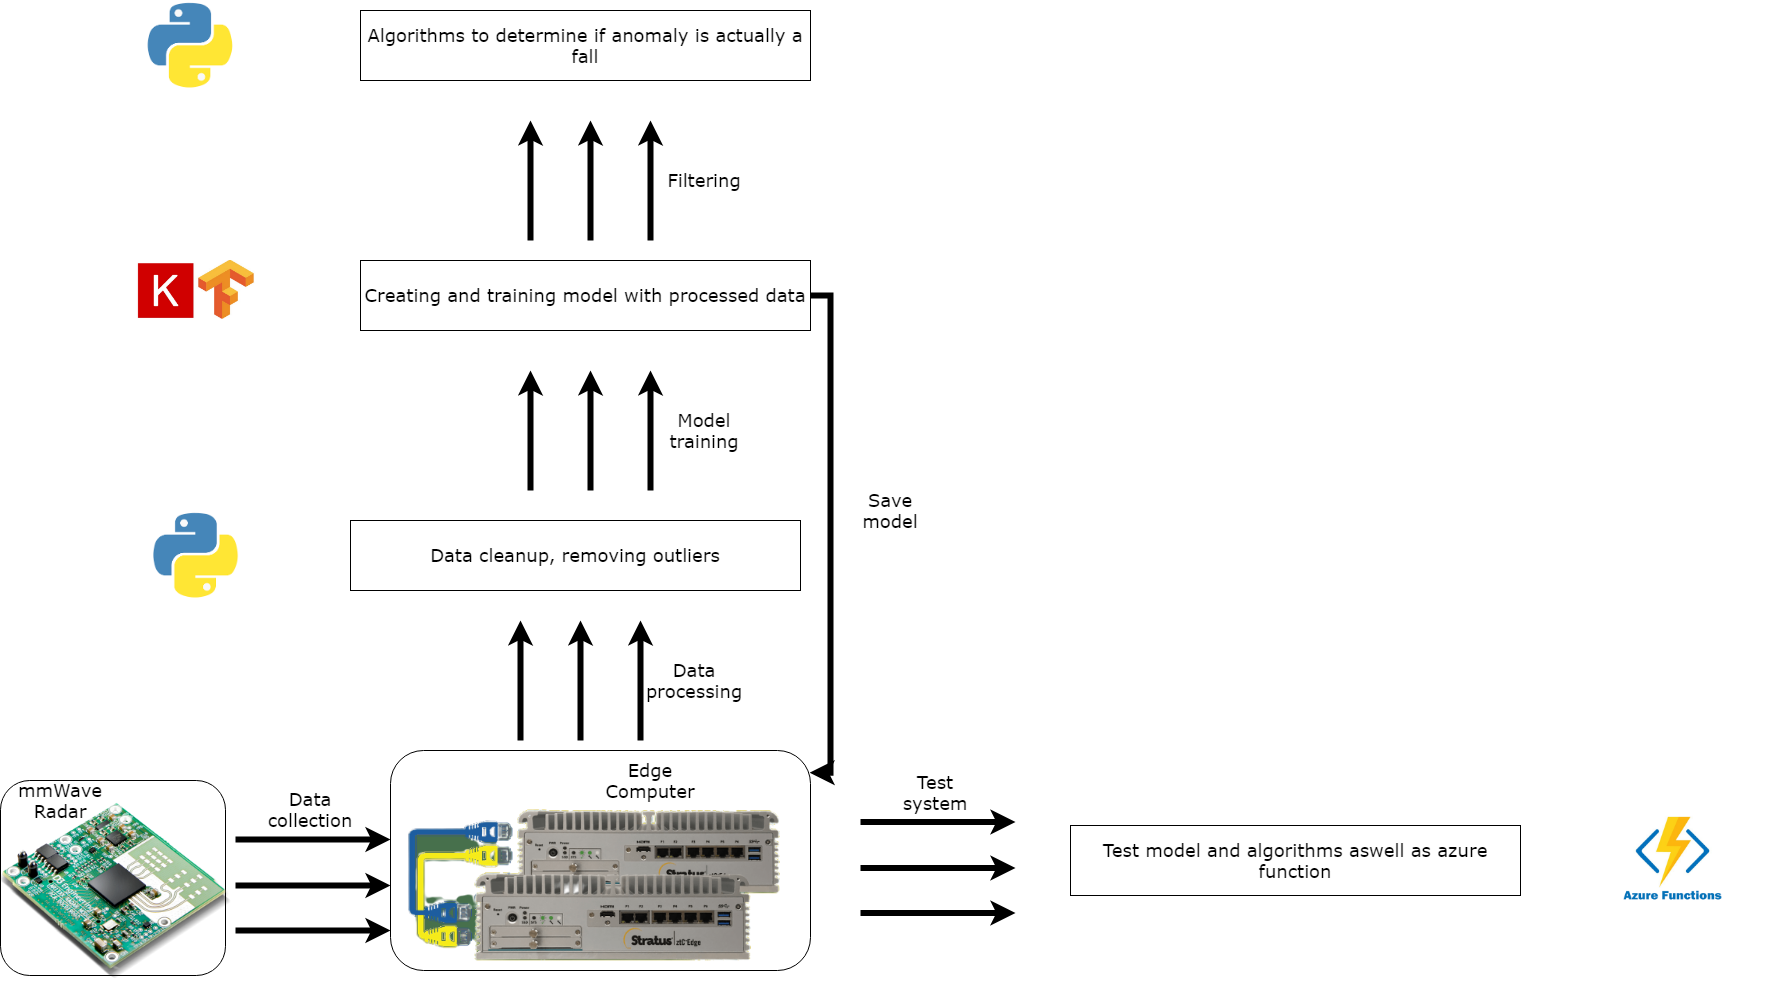
\includegraphics[width=400px, keepaspectratio]{archtrain.png}
    \vspace{1ex}%
    \caption{Architecture used for training the model.}
    \label{fig:my_label}
\end{figure}

\begin{figure}[H]
    \centering
    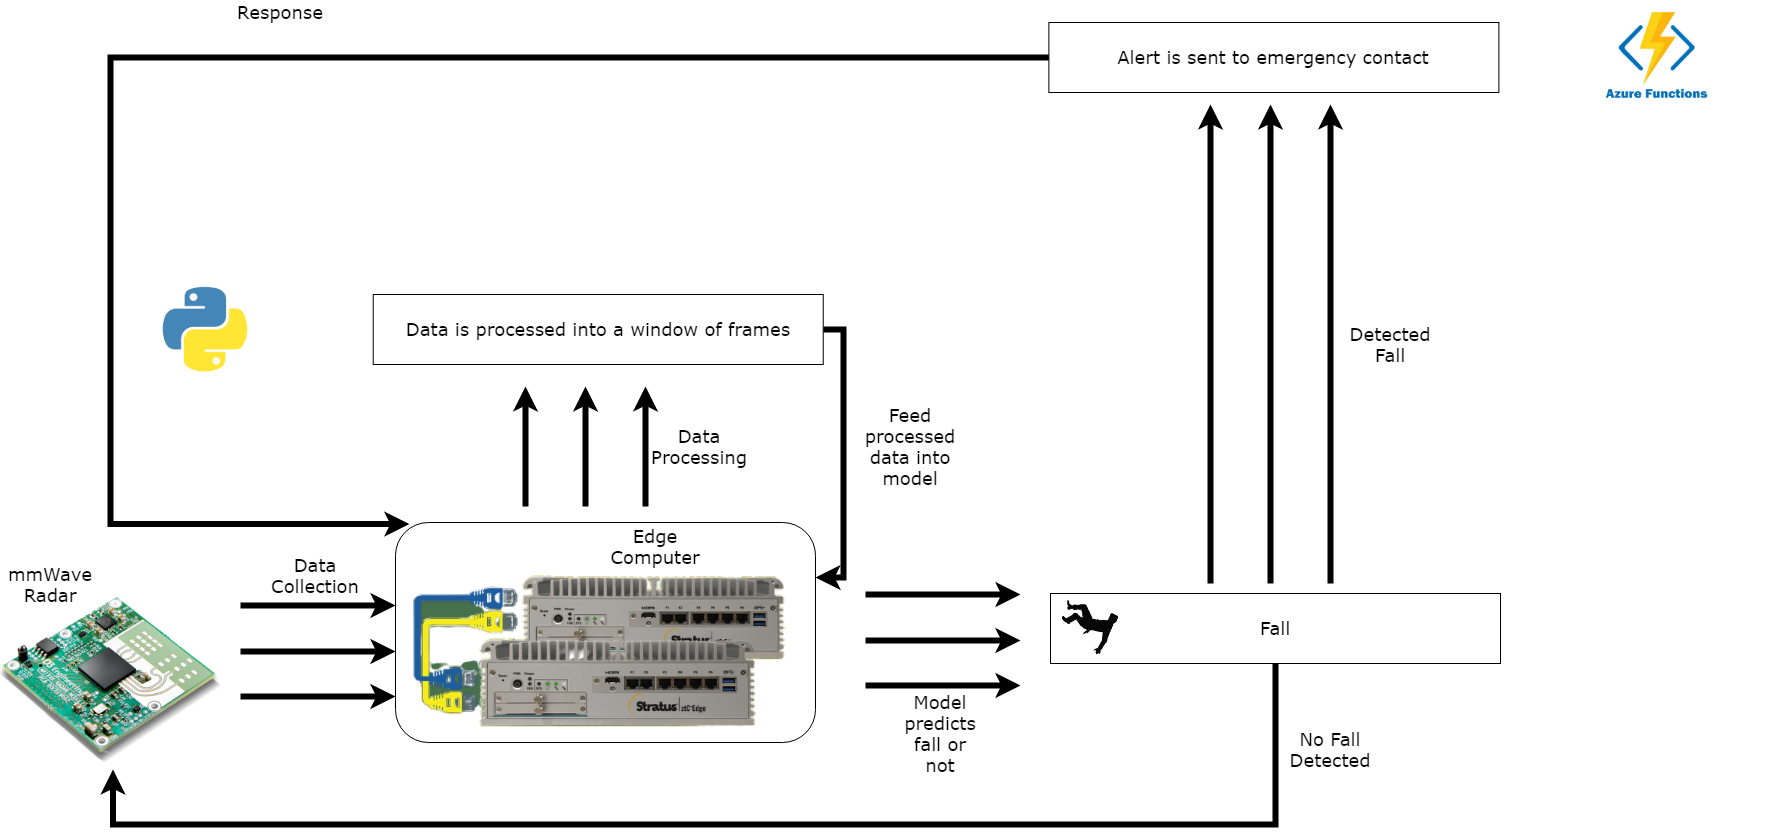
\includegraphics[width=400px, keepaspectratio]{archrealtime.png}
    \vspace{1ex}%
    \caption{Architecture used for real time detection.}
    \label{fig:my_label}
\end{figure}